\documentclass[12pt]{article}
\usepackage[a4paper,margin=0.8in]{geometry} % 明確設定四邊
\usepackage{fontspec}
\usepackage{xeCJK}
\usepackage{titling} % 預設標題下移0.6in
\usepackage{amsmath} % 數學方程式
\usepackage{graphicx} %圖片
\usepackage{float} % 在導言區 ,讓圖片強制插在原地
\usepackage{xcolor} %字體加入顏色
\usepackage{hyperref} % 引入網址
\usepackage{physics} % 物理符號
\usepackage{wrapfig} % 文字環繞圖片

\setmainfont{Times New Roman}
\setCJKmainfont{Kaiti TC}

\setlength{\droptitle}{-1in} % 上移標題0.6in
\title{QUICK離散格式的延遲修正(有界格式)}
\author{4.assignment\_2.4.tex}
\begin{document} 
\maketitle 
一、空間二階精度QUICK離散格式的延遲修正
\noindent   延遲修正(DC修正):\\

\noindent 空間二階精度QUICK離散格式的延遲修正格式為:\\

{
    \centering
    在離散方程中,將各個有限體積的邊界中心點的傳輸變數的空間二階精度QUICK格式的反擴散通量$(ex : \psi(r_{f})\frac{1}{2}(T_{D} - T_{C}))$,令為($S_{1}$($Q$($D$一維穩態擴散對流方程)的(空間二階精度QUICK離散格式))的(延遲修正等右外源項)):$S_{u\ e}^{DC}$。\\
    其中,$S_{u\ e}^{DC}$的定義域為計算空間內的所有計算點(包括內點及邊界點)。
}

\vspace{0.7em}
\noindent 不可壓縮理想氣體的一維穩態擴散對流方程的一般離散格式為:
\begin{equation}
    \begin{split}
        &\mbox{對於計算點}p(i,j)\mbox{有:}\\
        &A_{e}\cdot T_{i+\frac{1}{2},j}\cdot u_{x\ i+\frac{1}{2},j}  -A_{w}\cdot T_{i-\frac{1}{2},j}\cdot u_{x\ i-\frac{1}{2},j} \\
        =&A_{e}\cdot \frac{\alpha_{i+1,j}+\alpha_{i,j}}{2}\cdot \frac{T_{i+1,j} - T_{i,j}}{\Delta x_{Ep}} - A_{w}\cdot \frac{\alpha_{i,j}+\alpha_{i-1,j}}{2}\cdot \frac{T_{i,j} - T_{i-1,j}}{\Delta x_{pW}}
    \end{split}
\end{equation}
\noindent 其中,上式的近似方法為:\\
\noindent (1)、($l$($A$($f$($p$計算點)的(邊界中心點))的(擴散係數))的(近似)):

取為($A'$($p$計算點)的(擴散係數))跟($A''$($D$($p$計算點)的(相鄰計算點))的(擴散係數))的平均:\\
\begin{equation}
    \begin{split}
        \alpha_{f} \approx \frac{\alpha_{p} + \alpha_{D}}{2}
    \end{split}
\end{equation}
\noindent (2)、($g$($G$($f$($p$計算點)的(邊界中心點))的(溫度梯度))的(近似)):

取為($C$($G$($f$($p$計算點)的(邊界中心點))的(溫度梯度))的(二階精度中心差分)):\\
\begin{equation}
\begin{split}
    \frac{\partial T}{\partial n}_{f} \approx \frac{T_{(i,j) + \vec{e_{n}}} - T_{(i,j)}}{x_{(i,j) + \vec{e_{n}}} - x_{(i,j)}}
\end{split}
\end{equation}

\noindent 而(3)對:($T$($\phi$($f$($p$計算點)的(邊界中心點))的(傳輸變數))的(空間二階精度QUICK格式))取為:\\
\begin{equation}
    \begin{split}
        T_{i+\frac{1}{2},j} = T_{i,j} + (\frac{3}{8}T_{i+1,j} - \frac{2}{8}T_{i,j} - \frac{1}{8}T_{i-1,j})\ ; F_{e} > 0 \\
        T_{i-\frac{1}{2},j} = T_{i-1,j} + (\frac{3}{8}T_{i,j} - \frac{2}{8}T_{i-1,j} - \frac{1}{8}T_{i-2,j})\ ; F_{w} > 0 \\
    \end{split}
\end{equation}
\noindent 東邊界\\
\noindent 其中,上式的反擴散通量分別為:$\psi(r_f)\cdot \frac{T_{D} - T_{C}}{2}$ : \\
\noindent (a.) ($d'$($S$($T$($e$($p$計算點)的(東邊界中心點))的(傳輸變數))的(空間二階精度QUICK格式))的(反擴散通量)) : \\
\begin{equation}
    \begin{split}
        \phi_{QUICK\ i+\frac{1}{2},j}^{-1} = \frac{3}{8}T_{i+1,j} - \frac{2}{8}T_{i,j} - \frac{1}{8}T_{i-1,j} \\
    \end{split}
\end{equation}

\noindent (b.) ($d$($S$($T$($e$($p$計算點)的(東邊界中心點))的(傳輸變數))的(空間二階精度QUICK格式))的(擴散通量)) : \\
\noindent *擴散通量為不分格式,為空間一階精度upwind格式。\\
\begin{equation}
    \begin{split}
        \phi_{ i+\frac{1}{2},j}= T_{i,j} \\
    \end{split}
\end{equation}

\noindent (c.)($g'$($h$($H$($w$($p$計算點)的(西邊界中心點))的(傳輸變數))的(空間二階精度QUICK格式))的(反擴散通量)):\\
\begin{equation}
    \begin{split}
        \phi_{QUICK\ i-\frac{1}{2},j}^{-1} = \frac{3}{8}T_{i,j} - \frac{2}{8}T_{i-1,j} - \frac{1}{8}T_{i-2,j} \\
    \end{split}
\end{equation}

\noindent (d.) ($g$($h$($H$($w$($p$計算點)的(西邊界中心點))的(傳輸變數))的(空間二階精度QUICK格式))的(反擴散通量)) : \\
\noindent *擴散通量為不分格式,為空間一階精度upwind格式。\\
\begin{equation}
    \begin{split}
        \phi_{ i-\frac{1}{2},j}= T_{i-1,j} \\
    \end{split}
\end{equation}
\noindent 構造方法為:\\

在($W$($O$一維穩態擴散對流方程)的(空間二階精度QUICK離散格式))中,將\\

(1)($d'$($t$($T$($e$($p$計算點)的(東邊界中心點))的(傳輸變數))的(空間二階精度QUICK格式))的(反擴散通量))\\且

(2)($g'$($h$($H$($w$($p$計算點)的(西邊界中心點))的(傳輸變數))的(空間二階精度QUICK格式))的(反擴散通量))\\

令為($S_{1}$($Q$($D$一維穩態擴散對流方程)的(空間二階精度QUICK離散格式))的(延遲修正等右外源項))且($S_{2}$($Q$($D$一維穩態擴散對流方程)的(空間二階精度QUICK離散格式))的(延遲修正等右外源項))\\
則形成:\\

($D$($W$($O$一維穩態擴散對流方程)的(空間二階精度QUICK離散格式))的(延遲修正格式))

\begin{center}
    若且唯若$$A_{e}\cdot u_{x\ i+\frac{1}{2},j}\cdot \phi_{QUICK\ i+\frac{1}{2},j}^{-1} \rightarrow S_{u\ e
    }^{DC}$$ 
    $$A_{w}\cdot u_{x\ i-\frac{1}{2},j}\cdot \phi_{QUICK\ i-\frac{1}{2},j}^{-1} \rightarrow S_{u\ w}^{DC}$$
    則:$$Equation_{QUICK\ i,j} \rightarrow Equation_{QUICK\ i,j}^{DC}$$
\end{center}
\begin{figure}[H]
  \centering
  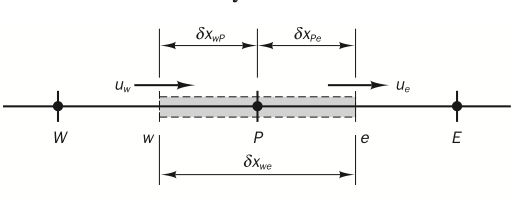
\includegraphics[scale = 1.2]{9.png}
  \caption{QUICK為三點格式,此為計算點$p$的一維有限體積}
  \label{fig:finite volume}
\end{figure}
\noindent 即有:\\

\noindent 若且唯若
    (1) \begin{center}($d'$($t$($T$($e$($p$計算點)的(東邊界中心點))的(傳輸變數))的(空間二階精度QUICK格式))的(反擴散通量))\end{center}
    被定義為
\begin{center}($S_{1}$($Q$($D$一維穩態擴散對流方程)的(空間二階精度QUICK離散格式))的(延遲修正等右外源項))\end{center}
\noindent 則:
\begin{center}($Q$($D$一維穩態擴散對流方程)的(空間二階精度QUICK離散格式))\end{center}
    被定義為
\begin{center}($E'$($Q$($D$一維穩態擴散對流方程)的(空間二階精度QUICK離散格式))的(延遲修正格式))\end{center}

\noindent (一)、內點所滿足的延遲修正格式:\\

\noindent 一般形式下的離散方程為:(對於計算點$(i,j)$)\\
\begin{equation}
    \begin{split}
        &A_{e}\cdot u_{x\ i+\frac{1}{2},j}(T_{QUICK\ i+\frac{1}{2},j} + T_{QUICK\ i+\frac{1}{2},j}^{-1}) - A_{w}\cdot u_{x\ i-\frac{1}{2},j}(T_{QUICK\ i-\frac{1}{2},j} + T_{QUICK\ i-\frac{1}{2},j}^{-1})\\
        =&\alpha(T_{i+1,j} - T_{i,j}) - \alpha(T_{i,j} - T_{i-1,j})
    \end{split}
\end{equation}

\noindent 將\begin{center}傳輸通量的離散取值的反擴散通量:$A_{e}\cdot u_{x\ i+\frac{1}{2},j}(T_{QUICK\ i+\frac{1}{2},j}^{-1})$移至等式右側,令為離散方程的延遲修正等右外源項:$S_{u\ e}^{DC}$\end{center}
同理,將\begin{center}傳輸通量的離散取值的反擴散通量:$A_{w}\cdot u_{x\ i-\frac{1}{2},j}(T_{QUICK\ i-\frac{1}{2},j}^{-1})$移至等式右側,令為離散方程的延遲修正等右外源項:$S_{u\ w}^{DC}$\end{center},則有:\\
\begin{equation}
    \begin{split}
        & A_{e}\cdot u_{x\ i+\frac{1}{2},j}(T_{i,j}) - A_{w}\cdot u_{x\ i-\frac{1}{2},j}(T_{i-1,j}) - \alpha (T_{i+1,j} -2\cdot T_{i,j} + T_{i-1,j}) \\
        = & - A_{e}\cdot u_{x\ i+\frac{1}{2},j}(T_{QUICK\ i+\frac{1}{2},j}^{-1}) + A_{w}\cdot u_{x\ i-\frac{1}{2},j}T_{QUICK\ i-\frac{1}{2},j}^{-1}
    \end{split}
\end{equation}
\noindent 對於各個內點$p$,則有(寫成符號形式):(對於計算點(範圍:i = 2 : Nx-1))\\
\begin{equation}
    \begin{split}
        &T_{p}(a_{W} + a_{E} - F_{w} + F_{e})\\
         = &a_{W}T_{W} + a_{E}T_{E} - S_{u\ e}^{DC}+ S_{u\ w}^{DC} 
    \end{split}
\end{equation}
\noindent 其中,
\begin{equation}
\begin{split}
    F_{w} &= A_{w}\cdot u_{x\ i-\frac{1}{2},j} \quad:\quad D_{w} = \alpha\\
    F_{e} &= A_{e}\cdot u_{x\ i+\frac{1}{2},j} \quad:\quad D_{e} = \alpha \\
    a_{W} &= D_{w} + F_{w} \\
    a_{E} &= D_{e} \\
    S_{u\ e}^{DC} &= F_{e}\cdot T_{QUICK\ i+\frac{1}{2},j}^{-1} = A_{e} \cdot u_{x\ i+\frac{1}{2},j}(T_{QUICK\ i+\frac{1}{2},j}^{-1}) \\
    S_{u\ w}^{DC} &= F_{w}\cdot T_{QUICK\ i-\frac{1}{2},j}^{-1} = A_{w} \cdot u_{x\ i-\frac{1}{2},j}(T_{QUICK\ i-\frac{1}{2},j}^{-1}) \\
    &\mbox{上二式均為計算點(範圍:i = 2 : Nx-1)的此離散方程的延遲修正等右外源項}\\
\end{split}
\end{equation}
\newpage
\vspace{-0.5cm}

\noindent (二)、左邊界第二排計算點\\

\noindent ($d$($f$($F$一維擴散對流方程)的(空間二階精度QUICK離散格式))的(DC修正格式)):(對於左邊界第二排計算點(範圍:i = 1))
\begin{equation}
    \begin{split}
        &A_{e}\cdot u_{x 1+\frac{1}{2},j}T_{1,j}-A_{w}\cdot u_{x\ 1-\frac{1}{2},j}T_{0,j} - \alpha(T_{2,j}-2T_{1,j}+T_{0,j})\\
        =& -A_{e} \cdot u_{x\ 1+\frac{1}{2},j}(\frac{3}{8}T_{2,j} - \frac{2}{8}T_{1,j} - \frac{1}{8}T_{0,j})+A_{w}\cdot u_{x\ 1-\frac{1}{2},j}(\frac{3}{8}T_{1,j} - \frac{1}{8}T_{0,j} - \frac{2}{8}T_{-\frac{1}{2},j})
    \end{split}
\end{equation}
\noindent 上式也可以寫成:\\
\begin{equation}
    \begin{split}
        &T_{p}(a_{W} + a_{E} - F_{w} + F_{e})\\
         = &a_{W}T_{W} + a_{E}T_{E} - S_{u\ w}^{DC\ *} + S_{u\ e}^{DC}
    \end{split}
\end{equation}
其中,對於計算點(範圍:i = 1),有:
\begin{equation}
\begin{split}
    F_{e} &= A_{e}\cdot u_{x\ 1+\frac{1}{2},j} \quad;\quad D_{e} = \alpha\\
    F_{w} &= A_{w}\cdot u_{x\ 1-\frac{1}{2},j} \quad;\quad D_{w} = \alpha\\
    a_{W} &= D_{w} + F_{w} \\
    a_{E} &= D_{e}\\
    S_{u\ e}^{DC} &= F_{e}\cdot T_{QUICK\ 1+\frac{1}{2},j}^{-1} = (\frac{3}{8}T_{2,j} - \frac{2}{8}T_{1,j} - \frac{1}{8}T_{0,j})\\
    S_{u\ w}^{DC\ *} &= F_{w}\cdot T_{QUICK\ 1-\frac{1}{2},j}^{-1} = (\frac{3}{8}T_{1,j} - \frac{1}{8}T_{0,j} - \frac{2}{8}T_{-\frac{1}{2},j}) \\
    &\mbox{上二式均被定義為計算點(範圍:i=1)的此離散方程的延遲修正等右外源項}\\
\end{split}
\end{equation}

\noindent (三)、左邊界計算點\\

\noindent ($d'$($f'$($F'$一為擴散對流方程)的(空間二階精度QUICK離散格式))的(DC修正格式)):(對於左邊界計算點(範圍:i = 0))\\
\begin{equation}
\begin{split}
    &A_{e}\cdot u_{x\ \frac{1}{2},j}T_{0,j} - 0  \\
    -&\alpha(T_{1,j}-T_{0,j}) + 0  \\
    -&A_{w}\cdot u_{x\ \frac{1}{2},j}T_{-\frac{1}{2},j}+ 2\alpha(T_{0,j} - T_{-\frac{1}{2},j})\\
    =& - A_{e}\cdot u_{x\ \frac{1}{2},j}(\frac{3}{8}T_{1,j} -\frac{1}{8}T_{2,j} - \frac{2}{8}T_{-\frac{1}{2},j}) + 0 
\end{split}
\end{equation}
\noindent 上式也可以寫成:\\
\begin{equation}
\begin{split}
    &T_{p}((a_{W}^{*}+a_{E}+F_{e})+S_{ul}^{*} - F_{w})\\
    =& a_{W}^{*}T_{W} + a_{E}T_{E} - S_{u\ e}^{DC\ *} + S_{u\ w}^{DC *}+ S_{ul}^{*}T_{-\frac{1}{2},j}
\end{split}
\end{equation}
\noindent 其中,對於左邊界計算點計算點(i = 0),有:\\
\begin{equation}
\begin{split}
    F_{e} &= A_{e}\cdot u_{x\ 1+\frac{1}{2},j} \quad;\quad D_{e} = \alpha\\
    F_{w} &= A_{w}\cdot u_{x\ 1-\frac{1}{2},j} \quad;\quad D_{w}^{*} = 2\alpha \\
    a_{W}^{*} &= 0\\
    a_{E} &= D_{e}\\
    S_{ul}^{*} &= D_{w}^{*} + F_{w} = 2\alpha + A_{w}u_{x\ -\frac{1}{2},j}\\
    &\mbox{上式即為左邊界計算點的此離散方程的等右外源項}\\
    S_{u\ e}^{DC *} &=  A_{e}u_{x\ \frac{1}{2},j}T_{QUICK\ \frac{1}{2},j}^{-1} = A_{e}u_{x\ \frac{1}{2},j}(\frac{3}{8}T_{1,j} - \frac{1}{8}T_{0,j} - \frac{2}{8}T_{-\frac{1}{2},j})\\
    S_{u\ w}^{DC *} &=  A_{w}u_{x\ -\frac{1}{2},j}T_{QUICK\ -\frac{1}{2},j}^{-1} = 0 \\
    &\mbox{上二式均被定義為左邊界計算點的此離散方程的延遲修正等右外源項}\\
\end{split}
\end{equation} 

\noindent (四)、右邊界計算點\\

\noindent ($d''$($f''$($F''$一維擴散對流方程)的(空間二階精度QUICK離散格式))的(DC修正格式)):(對於右邊界計算點(i = Nx-1))\\
\begin{equation}\begin{split}
    &0 - A_{w}\cdot u_{x\ Nx-1-\frac{1}{2},j}T_{Nx-2,j}\\
    -&0 + \alpha (T_{Nx-1,j} - T_{Nx-2,j})\\ 
    +&A_{e}u_{x\ Nx-\frac{1}{2},j}T_{Nx-\frac{1}{2},j}  - 2\alpha(T_{NX-\frac{1}{2},j} - T_{Nx-1,j})\\
    =& -0 + A_{w}u_{x\ Nx-1-\frac{1}{2},j}(\frac{3}{8}T_{Nx-1,j}- \frac{2}{8}T_{NX-2,j} - \frac{1}{8}T_{Nx-3,j})\\
    \end{split}
\end{equation}
\noindent 上式也可以寫成:\\
\begin{equation}
\begin{split}
        &T_{p}((a_{W}+a_{E}^{*}-F_{w}) + S_{ur}^{*} + F_{e})\\
        =&a_{W}T_{W} + a_{E}^{*}T_{E} - S_{u\ e}^{DC\ *} + S_{u\ w}^{DC} + S_{ur}^{*}T_{Nx-\frac{1}{2},j}\\
\end{split}
\end{equation}
\noindent 其中,對於右邊界計算點計算點(i = Nx-1),有:\\
\begin{equation}
    \begin{split}
        F_{w} &= A_{w}\cdot u_{x\ Nx-1-\frac{1}{2},j}\quad;\quad D_{w} = \alpha \\
        F_{e} &= A_{e}\cdot u_{x\ Nx-\frac{1}{2},j} \quad;\quad D_{e}^{*} = 2\alpha \\
        a_{W} &= D_{w}+F_{w} \\
        a_{E}^{*} &= 0 \\
        S_{ur}^{*} &= D_{e}^{*} - F_{e} = 2\alpha - A_{e}\cdot u_{x\ Nx-\frac{1}{2},j}\\
        &\mbox{上式即為右邊界計算點的離散方程的等右外源項}\\
        S_{u\ w}^{DC} &= F_{w}\cdot T_{QUICK\ Nx-1-\frac{1}{2},j}^{-1} = A_{w}u_{Nx-1-\frac{1}{2},j}\cdot (\frac{3}{8}T_{Nx-1,j} - \frac{2}{8}T_{Nx-2,j} - \frac{1}{8}T_{Nx-3,j})\\
        S_{u\ e}^{DC\ *} &= 0 \\
        &\mbox{上二式被定義為右邊界計算點的離散方程的延遲修正等右外援項}\\
    \end{split}
\end{equation}
\newpage
(五)、特殊處理\\
\noindent 
(1).\\
\begin{equation}
\begin{split}
    &a_{W} = D_{w} + F_{w} \quad;\quad for (i = 1 : Nx-1)\\
    &a_{W}^{*} = 0 \quad;\quad for(i = 0)\\
\end{split}
\end{equation}
(2).
\begin{equation}
\begin{split}
    &a_{E} = D_{e} \quad;\quad for (i = 0 : Nx-2)\\
    &a_{E}^{*} = 0\quad;\quad for(i = Nx-1 )\\
\end{split}
\end{equation}
(3).
\begin{equation}
\begin{split}
    &S_{ul}^{*} = D_{w}^{*} + F_{w}  = 2\alpha + A_{w}u_{i-\frac{1}{2},j}\quad;\quad for (i = 0)\\
    &S_{ur}^{*} = D_{e}^{*} - F_{e} = 2\alpha - A_{e}\cdot u_{x\ Nx-\frac{1}{2},j}\\
\end{split}
\end{equation}
(4).
\begin{equation}
\begin{split}
    &D_{w} = \alpha \quad;\quad for(i = 1 ; Nx-1)\\
    &D_{w}^{*} = 2\alpha\quad;\quad for (i = 0)\\
    &D_{e} = \alpha \quad;\quad for(i = 0 : Nx-2)\\
    &D_{e}^{*} = 2\alpha \quad;\quad for(i = Nx-1)\\
\end{split}
\end{equation}
(5).
\begin{equation}
\begin{split}
    &S_{u\ w}^{DC} = A_{w}u_{x\ i-\frac{1}{2},j}(\frac{3}{8}T_{i,j} - \frac{2}{8}T_{i-1,j} - \frac{1}{8}T_{i-2,j})  \quad;\quad for (i = 2 : Nx-1)\\
    &S_{u\ w}^{DC\ *} = 0 \quad;\quad for (i = 0)\\
    &S_{u\ w}^{DC\ *} = A_{w}u_{x\ 1-\frac{1}{2},j}(\frac{3}{8}T_{1,j} - \frac{1}{8}T_{0,j} - \frac{2}{8}T_{-\frac{1}{2},j}) \quad;\quad for (i = 1)\\
    &S_{u\ e}^{DC\ } = A_{e}u_{x\ i+\frac{1}{2},j}(\frac{3}{8}T_{i+1,j} - \frac{2}{8}T_{i,j} - \frac{1}{8}T_{i-1,j}) \quad;\quad for (i = 1 : Nx-2)\\
    &S_{u\ e}^{DC\ *} = A_{e}u_{x\ 1-\frac{1}{2},j}(\frac{3}{8}T_{1,j} - \frac{1}{8}T_{0,j} - \frac{2}{8}T_{-\frac{1}{2},j}) \quad;\quad for(i = 0)\\
    &S_{u\ e}^{DC\ *} = 0  \quad;\quad for(i = Nx-1)\\
\end{split}
\end{equation}
\end{document}


